\documentclass{article}

\pdfoutput=1

\usepackage{amsmath}
\usepackage{amsfonts}
\usepackage{mathtools}
\usepackage{algorithm}
\usepackage{algorithmicx}
\usepackage{algpseudocodex}
\usepackage{graphicx}
\usepackage[margin=1in]{geometry}

\graphicspath{{figures/}}

\DeclareMathOperator*{\argmin}{arg\,min}

\title{A Tool for Visualizing and Analyzing High-Dimensional Clustering Performance}
\author{Justin Lin\footnote{Department of Mathematics, Indiana University} and Julia Fukuyama\footnote{Department of Statistics, Indiana University}}
\date{}

\begin{document}
\maketitle

\abstract{Technological advances have spurred an increase in data complexity and dimensionality. We are now in an era in which data sets containing thousands of features are commonplace. To digest and analyze such high-dimensional data, dimension reduction techniques have been developed and advanced along with computational power. Of these techniques, nonlinear methods are most commonly employed because of their ability to construct visually interpretable embeddings. Unlike linear methods, these methods non-uniformly stretch and shrink space to create a visual impression of the high-dimensional data. Since capturing high-dimensional structures in a significantly lower number of dimensions requires drastic manipulation of space, nonlinear dimension reduction methods are known to occasionally produce false structures, especially in noisy settings. In efforts to deal with this phenomenon, we developed an interactive tool that enables analysts to better understand and diagnose their dimension reduction results. It uses various analytical plots to provide a multi-faceted perspective on results to determine legitimacy. The tool is available via an R package named \textit{DRtool}.}

\section{Introduction}
The potency of nonlinear dimension reduction methods lies in their flexibility, allowing them to model complex data structures. That same flexibility, however, makes them difficult to use and interpret. Each method requires a slew of hyperparameters that need to be calibrated, and even when adequately calibrated, these methods require a trained eye to interpret. For example, the two most popular nonlinear dimension reduction methods, t-SNE and UMAP, are known to generate unintuitive results (\cite{understanding UMAP}, \cite{Distill}). The results often cluster, even when no clusters exist in the data, and cluster sizes/placements can be unreliable. We've developed an interactive tool that analysts may use to conduct a post-hoc analysis of their high-dimensional clustering. The tool uses the minimum spanning tree (MST) to model the global structure of clusters and provide an additional perspective on inter-cluster relationships. This allows analysts to extract more information from their dimension reduction results by making it easier to differentiate the signal from the noise.

In this paper, we describe the analytical plots provided by the tool (Section 2). We present a MST stability experiment, demonstrating the MST's ability to approximate high-dimensional structure (Section 3). And we walk through use of the tool on an image data set and a mass cytometry data set (Section 4).

\section{Methods}

\subsection{The Minimum Spanning Tree}
Graphs have been applied to many multivariate statistical problems. The authors of \cite{MAP test} introduced the minimal ascending path spanning tree as a way to test for multimodality. The Friedman-Rafsky test \cite{Friedman-Rafsky test}, along with its modern variations \cite{Friedman-Rafsky variation 1, Friedman-Rafsky variation 2, Friedman-Rafsky variation 3}, use the MST to construct a multivariate two-sample test. Single-linkage clustering \cite{single-linkage and MST} and runt pruning \cite{runt pruning} are both intimately related with the MST. In the context of dimension reduction, IsoMap \cite{IsoMap} makes use of neighborhood graphs, \cite{MIST example} introduces the maximum information spanning tree, and \cite{MST example} uses the MST. These methods, which fall under the category of manifold learning, use graphs to model high-dimensional data assumed to be drawn uniformly from a high-dimensional manifold. An accurate low-dimensional embedding can then be constructed from these graphs. It's apparent that graphs are useful for modeling high-dimensional data, especially when it comes to dimension reduction and cluster analysis. Our tool uses the MST to analyze the reliability of visualizations produced by nonlinear dimension reduction methods.

We've opted for the MST for a couple of key properties. Firstly, the MST and shortest paths along it are quick to compute. Secondly, the MST contains a unique path between any two vertices, providing a well-defined metric on the data. Lastly, it provides a good summary of the data's structure. It contains as a subgraph the nearest-neighbor graph, and any edge deletion in the MST partitions the vertices into two sets for which the deleted edge is the shortest distance between them \cite{Friedman-Rafsky test}.

\subsubsection{MST Stability}
The MST is meant to provide a robust estimation of the data's global structure, and more specifically, inter-cluster relationships. As such, it should be stable in the presence of noise and unaffected by local transformations of the data. To demonstrate MST stability, we study the effect of random noise on the inter-cluster relationships explained by the MST.

To derive the inter-cluster relationships from the MST, we simplified the medoid subtree using the following procedure:

\begin{algorithm}[H]
\caption{Simplified Medoid Subtree}\label{algo1}
\begin{algorithmic}[1]
\Require MST $T = (V, E)$ with cluster medoids $m_1, \hdots, m_k \in V$
\State $T' = (V', E') \Leftarrow$ minimal subtree of $T$ containing all $m_i$
\Repeat
	\State Let $v \in V' \setminus \{m_1,  \hdots, m_k\}$ with $deg(v) = 2$ and neighbors $a, b \in V'$. Let $d(v, a)$ and $d(v, b)$ be the weights of the edges incident to $v$.
	\State Replace $v$ and its two incident edges with an edge connecting $a$ and $b$ with weight $d(v, a) + d(v, b)$.
\Until{$T'$ no longer contains non-medoid vertices with degree two.}
\State \Output T'
\end{algorithmic}
\end{algorithm}

The simplification process essentially replaces paths of non-medoid vertices with one edge of equal length. We refer to this tree as the simplified medoid subtree. It encode global inter-cluster relationships within the data.

\subsubsection{Robinson-Foulds Metric}
To compare simplified medoid subtrees, we used the Robinson-Foulds metric \cite{RF metric}. The R-F metric was originally introduced to quantify the dissimilarity of phylogenetic trees, but the algorithm generalizes to arbitrary weighted trees. It looks at partitions of each tree created by removing individual edges, then counts the number of partitions present in one tree but not in the other. We modified the algorithm (Algorithm 2) to specifically measure the dissimilarity in medoid vertices.

\begin{algorithm}[H]
\caption{Robinson-Foulds Distance}\label{algo2}
\begin{algorithmic}[2]
\Require Trees $T_1 = (V_1,E_1)$ and $T_2 = (V_2, E_2)$ with medoids $m_1, \hdots, m_k \in V_1$ and $n_1, \hdots, n_k \in V_2$
\State $P_1 \Leftarrow \{\}$
\For{$e \in E_1$}
	\State $G \Leftarrow (V_1, E_1 \setminus \{e\})$ with connected components $G_1$ and $G_2$
	\State $M_1 \Leftarrow \{m_1,\hdots,m_k\} \cap V(G_1)$
	\State $M_2 \Leftarrow \{m_1,\hdots,m_k\} \cap V(G_2)$
	\State $P_1 \Leftarrow \Call{Add}{P_1, \{M_1, M_2\}}$
\EndFor
\State $P_2 \Leftarrow \{\}$
\For{$e \in E_2$}
	\State $G \Leftarrow (V_2, E_2 \setminus \{e\})$ with connected components $G_1$ and $G_2$
	\State $M_1 \Leftarrow \{n_1,\hdots,n_k\} \cap V(G_1)$
	\State $M_2 \Leftarrow \{n_1,\hdots,n_k\} \cap V(G_2)$
	\State $P_2 \Leftarrow \Call{Add}{P_2, \{M_1, M_2\}}$
\EndFor
\State \Output $\frac{\left|P_1 \Delta P_2 \right|}{2\left| P_1 \cap P_2 \right|}$
\end{algorithmic}
\end{algorithm}

\subsection{The Tool}
The main objective is to analyze and leverage the structural data embedded in the MST. For example, paths between clusters are used to study inter-cluster relationships in the context of the underlying manifold from which the data is drawn.

To start, the user must provide, at the very least, a data matrix, a low-dimensional embedding, and a clustering. From there, the MST is calculated and various analytical plots are provided. The primary plot is the low-dimensional embedding colored according to the provided clustering. There is an option to overlay the medoid MST to understand the global structure of the clusters. The medoid MST is the minimal subtree of the MST containing the medoid of each cluster.

The remaining plots require the user to select two groups of interest, which can be done interactively in one of two ways. One way is to select two endpoints. The MST path is calculated and projected onto the low-dimensional-embedding. The two groups are then the classes each endpoint belongs to. The second way is to select custom groups. The user may interact with the low-dimensional by drawing boundaries for each group. The projected path then connects the medoid of each group. Once the groups and path are specified, the user is provided additional plots used to investigate the relationship between the two selected groups of points.

\subsection{Path Projection Plot}
To better understand the path of interest, a local projection method is applied to visualize the path and nearby points in two dimensions. The goal of the projection is to "unwind" the path, so that it can be used to study the relationship between the two selected groups. We apply Principal Component Analysis followed by regularized Canonical Correlation Analysis in a method we've dubbed the PCA -- rCCA method.

\subsubsection{The PCA -- rCCA Method}
Let $P \in \mathbb{R}^{k \times p}$ be the matrix of high-dimensional path points with endpoints $p_1, p_k \in \mathbb{R}^p$. Let $X \in \mathbb{R}^{n \times p}$ be the matrix of points of interest, i.e. the points belonging to one of the selected groups and the points along the path.

The concept is to use Canonical Correlation Analysis to determine the two-dimensional linear projection that best unwinds the path. Given two matrices, CCA iteratively calculates linear combinations of the matrix variates for each matrix, known as canonical variate pairs, that maximize covariance. These pairs are chosen to be orthogonal so that they give rise to a projection subspace. To unwind $P$, we use CCA to compare $P$ against the data matrix modeling a $d$-dimensional polynomial $$P_d = \begin{bmatrix}
1 & 1^2 & \cdots & 1^d \\
2 & 2^2 & \cdots & 2^d \\
\vdots & \vdots & & \vdots \\
n & n^2 & \cdots & n^d
\end{bmatrix}$$
and use the first two canonical variate pairs to construct a two-dimensional projection that maximizes the covariance between projections of $P$ and $P_d$. This process generates a two-dimensional subspace on which we can project all of $X$. Regularization is required to avoid singularity because $p$ is often much greater than $k$. The regularization constant for $P$ is chosen using cross-validation. No regularization constant is needed for $P_d$. See \cite{rCCA} for details.

One issue with this method is the projected path often travels along the outskirts of the plot. This is due to the near-orthogonality of high-dimensional data \cite{near-orthogonal}. Because the non-path points are often nearly orthogonal with the projection subspace, they are overly shrunk in the projection. The path points are less affected because the projection subspace is selected to retain the path's shape. While this phenomenon doesn't discredit the entire plot, it leads to misrepresentation of the path's location relative to the rest of the points.

To alleviate this issue, we apply PCA on the entirety of $X$ to prior to applying rCCA. Removing extraneous dimensions containing mostly noise prevents the confusion of excess noise for independence. When rCCA is applied post-PCA, the projected path's relative position to the rest of the points is more credible.

\subsection{MST Test}
Another perspective on the relationship between the two selected groups can be gained by studying their connectivity in the MST. More specifically, the number of MST crossings between the two groups is a measure of separation. A large number of crossings indicates lesser separation, while a small number of crossings indicates more separation. This idea motivates a hypothesis test.

\subsubsection{The Test Statistic}
The test statistic is the number of crossings between the two groups, which is counted according to the following procedure. The minimal subtree containing both groups is isolated. Because the two groups may not be adjacent in the MST, this subtree may contain other clusters as well. To extract the structural relationship between the two groups of interest, the subtree must be simplified. The simplification process includes condensing paths between points of non-points of interest into a single edge, then collapsing edges between non-points of interest (Algorithm 3).  This procedure essentially collapses paths between the two groups of interest into edges that can be counted.

\begin{algorithm}[H]
\caption{Simplify Subtree}\label{algo3}
\begin{algorithmic}[3]
\Require Tree $T = (V,E)$, group one vertices $V_1 \subset V$, and group two vertices $V_2 \subset V$
\State $T' = (V', E') \Leftarrow$ minimal subtree of $T$ containing $V_1 \cup V_2$
\Repeat
	\State Let $v \in V' \setminus (V_1 \cup V_2)$ with $deg(v) = 2$ and neighbors $a, b \in V'$. Let $d(v, a)$ and $d(v, b)$ be the weights of the edges incident to $v$.
	\State Replace $v$ and its two incident edges with an edge connecting $a$ and $b$ with weight $d(v, a) + d(v, b)$.
\Until{$T'$ no longer contains non-group vertices with degree two.}
\Repeat
	\State Let $v_1, v_2 \in V' \setminus (V_1 \cup V_2)$ be adjacent.
	\State Collapse the edge connecting $v_1$ and $v_2$. The combined vertex is adjacent to all neighbors of $v_1$ and $v_2$.
\Until{$T'$ no longer adjacent non-group vertices.}
\end{algorithmic}
\end{algorithm}

To count the number of crossings, the number of edges between the two groups in the simplified subtree are counted. It is also possible for a non-point of interest to act as a mediator along a path between the two groups of interest. To account for this scenario, for each non-point of interest adjacent to both groups, we also count its maximal degree to both groups.

\subsubsection{The Null Distribution}
The null distribution should represent the number of crossings in the case when both groups belong to the same cluster. Hence, we consider a uniform distribution on a hyperrectangle whose side lengths are proportional to the singular values of the appropriate cluster. The proportionality constant is $\sqrt{12}$, so the variances of this distribution in each principal direction are equal to the variances of the data in the direction of each principal component. Extraneous dimensions are also removed to reduce noise. Once the points are sampled, the MST is calculated, and the number of edges crossing a splitting hyperplane is recorded.

To determine the number of points to be sampled, we must consider the density of the data. This is a largely important decision as the number of edge crossings is determined by the local density near the splitting hyperplane. The many reasonable ways to determine the sample size, but to ensure our test has the correct size, we must select the sample size that maximizes the probability of rejection under the null hypothesis. That way, the null would also be rejected under any other reasonable sample size. The probability of rejection is maximized when the alpha quantile of the null distribution is minimized, i.e. when the simulated number of crossings is minimized. Therefore, we tune the sample size to match the lesser density between the two clusters.

The density of each cluster is approximated by the number of samples divided by the product of singular values after truncation $$D_i = \frac{n_i}{\prod_j \sigma_j^i} \textrm{ for } i=1,2.$$ If $i_0 = \argmin_i D_i$, then $n_{i_0}$ points are sampled from the hyperrectangle with side lengths $\sqrt{12}\sigma_j^{i_0}$. The simulation process yields an approximate distribution to which the test statistic is compared to. The p-value is the percentile of the test statistic within this simulated distribution. A 1-sided test is employed because we are only interested in rejecting the null given sufficiently small values of the test statistic.

\subsection{Heatmap}
The heatmap is a very useful tool for comparing groups because they provide a feature-by-feature perspective. It pinpoints the exact features in which the two groups differ the most. The interactive heat map also allows users to select and analyze sub-heatmaps, provided a more focused view on specific features.

\subsection{Meta Data Plot}
Along with the data and clustering, the user may also supply meta data corresponding to the samples in the original data. The meta data for each group is presented via pie charts for categorical data and box plots for numerical data. These plots are useful for discovering trends in the data.

\section{Results}

\subsection{MST Stability Experiment}
1,500 samples were randomly chosen from the MNIST data set of handwritten digits \cite{MNIST}. Each $28 \times 28$-pixel image was flattened into a vector of length $28^2 = 784$, so the data contain 1,500 samples in $784$ dimensions. A PCA pre-processing step was employed to reduce the number of dimensions to 300. The simplified medoid subtree $T$ was then calculated.

Random Gaussian noise was then added to the data and the new simplified medoid subtree $T'$ was calculated. The R-F distance $RF(T, T')$ was recorded. This process was repeated 30 times.

\renewcommand{\figurename}{Figure}
\renewcommand{\thefigure}{1}
\begin{figure*}[!t]
\centering
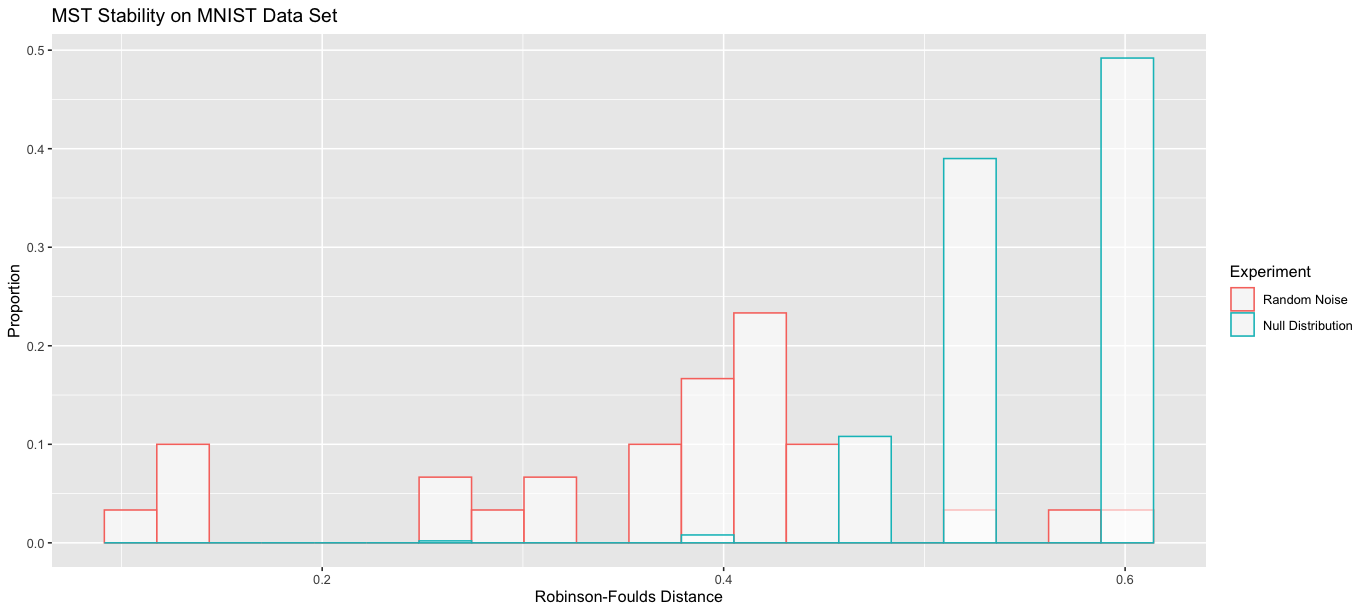
\includegraphics[scale=0.3]{RF stability}
\caption{MST Stability on MNIST Data Set}
\end{figure*}

To better interpret the R-F distances, we designed a null distribution of distances as a reference for comparison. These distances should represent R-F distances between trees that do not portray similar global structures and inter-cluster relationships. To generate the null distribution from the data, we randomly permuted the class labels and computed the R-F distances between the resulting simplified medoid subtrees and the original simplified medoid subtree. By randomly re-labelling the clusters, we are simulating examples with distinct global structures. Figure 1 shows the R-F distances produced by adding noise and permuting the class labels. The simplified medoid subtree trees generated by adding noise were significantly closer to the original simplified medoid subtree than those generated by randomly permuting the class labels in terms of R-F distance.

\section{Application}

\subsection{Image Data Example}
To demonstrate use of the tool, we explore the MNIST data set in detail. Again, the $784 \times 784$-pixel images were flattened and 1,500 samples were randomly sampled. A PCA pre-processing step was applied prior to applying UMAP \cite{UMAP} to construct a two-dimensional embedding. To replicate a real use case, we study a k-means clustering instead of the true class labels (Figure 2). The reader may follow along using the \texttt{run\_example(example="MNIST", cluster="kmeans")} function in our \textit{DRtools} package.

\renewcommand{\figurename}{Figure}
\renewcommand{\thefigure}{2}
\begin{figure*}[!t]
\centering
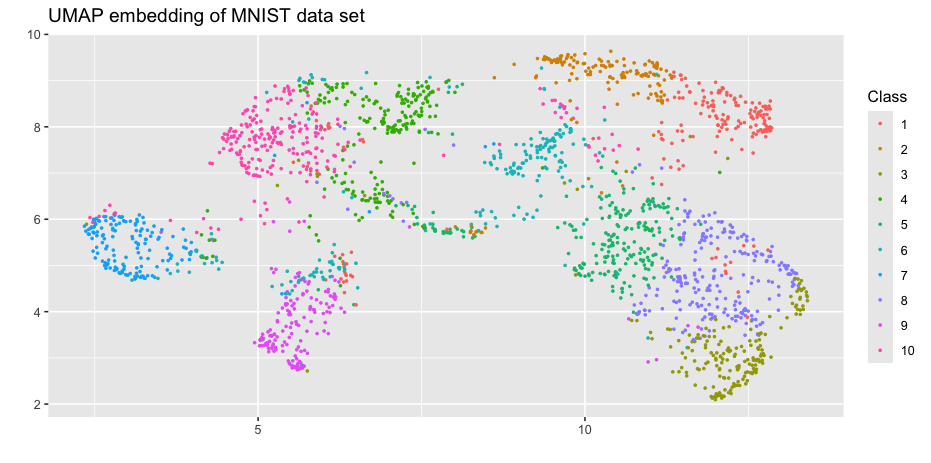
\includegraphics[scale=0.45]{MNIST kmeans}
\caption{MNIST Embedding with k-Means Coloring}
\end{figure*}

At first glance, there are two major instances of disagreement between the low-dimensional embedding and the k-means clustering. Classes 1 and 2 seem to form one cluster together, while class 4 is split into two separate clusters. Let's take a closer look.

\renewcommand{\figurename}{Figure}
\renewcommand{\thefigure}{3}
\begin{figure*}[!b]
\centering
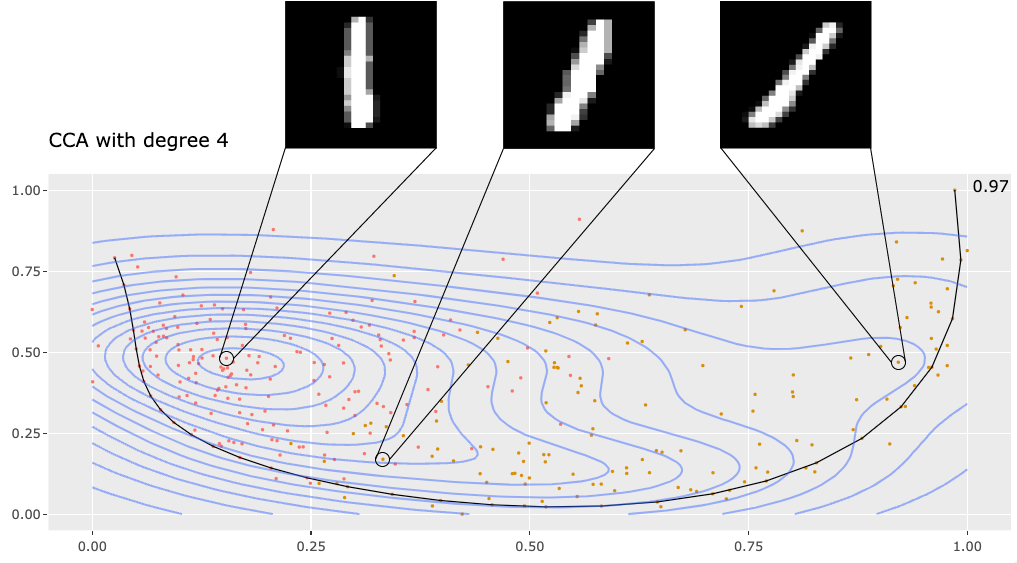
\includegraphics[scale=0.4]{class 1+2 projection}
\caption{Projection of Path Between Classes 1 and 2}
\end{figure*}

\subsubsection{Classes 1 and 2}
There seems to be minimal separation between classes 1 and 2, suggesting they may correspond to the same digit. We select a path from point 25,483 in class 1 to point 44,483 in class 2. To get a closer look, we first look at the Path Projection Plot. There are two settings that must be calibrated -- Dimension and CCA Degree. Dimension refers to the dimensionality of the PCA step. It is recommended to start with a modestly large number of dimensions, say 100 in our case, which still retaines 97\% of the variance. CCA Degree refers to the degree $d$ of the polynomial design matrix $P_d$ used during the rCCA step. To calibrate $d$, the user should start with $d = 2$ and increment $d$ until the shape of the path stabilizes, which occurs at $d = 4$ in our case.

The resulting plot depicts overlap between the two classes. Adjusting the bandwidth of the density estimate to 1.5 shows unimodal density, suggesting the two classes may come from the same population. Showing the MST edges also does not provide any evidence of separation. The MST test results, however, diverge. Only 18 crossings are counted when the approximate expectation under the null hypothesis is 26.45. The bootstrapped $p$-value of $0.04$ indicates the classes may come from distinct populations.

Inspection of the handwritten digits themselves reveals an interesting trend. While the majority of samples from both classes depict the digit one, the angle of the stroke differs drastically between the classes (Figure 2). Following the path from class 1 to class 2, the angle of the stroke becomes less and less steep. Both the MST path and MST test were able to detect this phenomenon.

Overall, the analytical plots provide context that the UMAP embedding alone does not. There is a gradual decline in density as you move across the combined cluster, which corresponds to increasingly slanted one digits. The MST test was able to detect the difference in penmanship, but the rather modest $p$-value of 0.04 well-represents the subtlety of the situation.

\renewcommand{\figurename}{Figure}
\renewcommand{\thefigure}{4}
\begin{figure*}[!b]
\centering
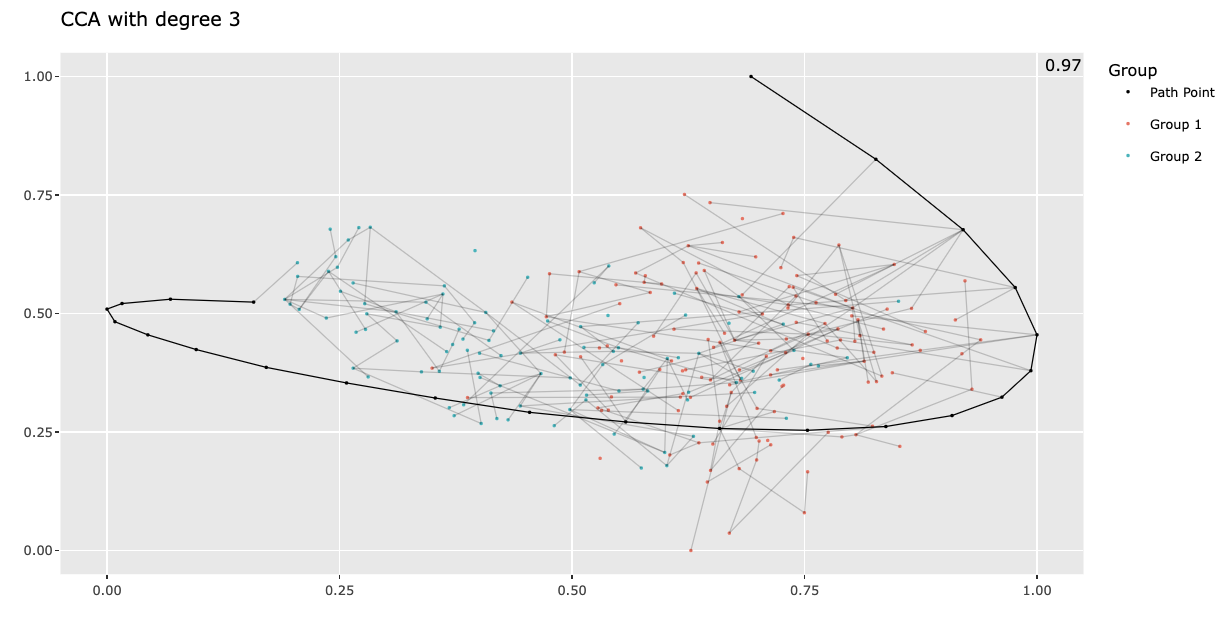
\includegraphics[scale=0.35]{class 4 projection}
\caption{Projection of Path Between Class 4 Clusters}
\end{figure*}

\subsubsection{Class 4}
Class 4 is split between two different clusters in the UMAP embedding. We use the drawing tool to select the two clusters as our groups. The path projection settings are calibrated to 100 dimensions and a CCA degree of three. We also select the Group Coloring setting so the points are colored according to group, rather than class. Analysis of the plot and estimated density does not provide evidence of separation. The MST edges, however, do. Close examination of the edges reveals a scarcity of inter-group edges (Figure 4). Even in overlapping regions, the edges tend to connect points belonging to the same group. This observation is confirmed by the MST test. Only 14 inter-group crossings are counted when the null distribution has expectation 20.56 and standard error 4.99, giving a bootstrapped $p$-value of 0.11. It is unsurprising that the MST was able to detect the separation, while the PCA -- rCCA projection was not. The MST accounts for the high-dimensional manifold from which the data is sampled, while the local PCA -- rCCA projection does not. Moreover, linear projections tend to compress the data, especially when the reduction in dimension is this drastic.

According to the true class labels, these clusters correspond to distinct digits. The top cluster, (group one) corresponds to the digit eight, while the bottom cluster (group two) corresponds to the digit five. It is certainly understandable how k-means was unable to distinguish these two digits.

\renewcommand{\figurename}{Figure}
\renewcommand{\thefigure}{5}
\begin{figure*}[!t]
\centering
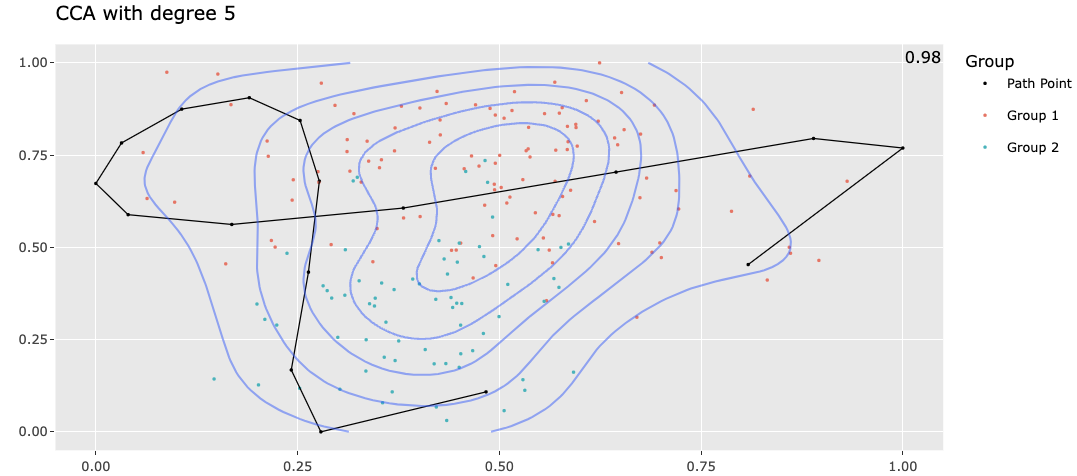
\includegraphics[scale=0.37]{class 9 projection}
\caption{Projection of Path Between Class 9 and Remainder of Cluster}
\end{figure*}

\subsubsection{Class 9}
Class 9 is well-separated, but its cluster also contains some points from other classes, mainly class 6. To determine if these points should belong to the same class, we use the drawing tool to select the class 9 points and the remaining points in the cluster as our groups. The path projection settings are calibrated to 100 dimensions and a CCA degree of five. Together, the points form a unimodal cluster, as shown by the approximate density calculated with a bandwidth of 1.3 (Figure 5). Visually, there is also a consistent density of MST edges throughout the cluster, even where the two groups meet. The MST test agrees. There are 16 crossings counted, just below the expected value 16.37 under the null hypothesis. All evidence points towards the merging of these two groups.

According to the true class labels, this entire cluster corresponds with the digit six. The k-means clustering incorrectly scattered the points into multiple classes.

\subsection{Mass Cytometry Data Set}
We now explore a mass cytometry data set \cite{Wong data set} covering 35 samples originating eight distinct human tissues enriched for T and natural killer cells. The data is processed and labeled according to the procedure laid out \cite{UMAP example}.

\newpage

\begin{thebibliography}{99}

\bibitem{fractional Lp norms}
Charu C. Aggarwal, Alexander Hinneburg, and Daniel A. Keim.
\newblock On the surprising behavior of distance metrics in high dimensional space.
\newblock {\em Lecture Notes in Computer Science, vol. 1973}, 2001.

\bibitem{UMAP example}
Becht et al.
\newblock Dimensionality reduction for visualizing single-cell data using UMAP.
\newblock {\em Nature Biotechnology 37:38-44}, 2019.

\bibitem{Friedman-Rafsky variation 1}
Bhaswar B. Bhattacharya.
\newblock A general asymptotic framework for distribution-free graph-based two-sample tests.
\newblock {\em Journal of the Royal Statistical Society Series B: Statistical Methodology 81:3, 575-602}, 2019.

\bibitem{Friedman-Rafsky variation 2}
Hao Chen and Jerome H. Friedman.
\newblock A new graph-based two-sample test for multivariate and object data.
\newblock {\em Journal of the American Statistical Association 112:517, 397-409}, 2017.

\bibitem{Friedman-Rafsky variation 3}
Hao Chen, Xu Chen, and Yi Su.
\newblock A weighted edge-count two-sample test for multivariate and object data.
\newblock {\em Journal of the American Statistical Association 113:523, 1146-1155}, 2018.

\bibitem{understanding UMAP}
Andy Coenen and Adam Pearce for Google PAIR.
\newblock Understanding UMAP.
\newblock {\em https://pair-code.github.io/understanding-umap/}.

\bibitem{MNIST}
Li Deng.
\newblock The MNIST database of handwritten digit images for machine learning research.
\newblock {\em IEEE Signal Processing Magazine 29:6}, 2012.

\bibitem{near-orthogonal}
Persi Diaconis and David Freedman.
\newblock Asymptotics of graphical projection pursuit.
\newblock {\em The Annals of Statistics 12:3, 783-815}, 1984.

\bibitem{image metrics}
Vito Di Ges\`u and Valery Starovoitov.
\newblock Distance-based functions for image comparison.
\newblock {\em Pattern Recognition Letters 20:2, 207-214}, 1999.

\bibitem{CCA package}
Gonz\'alez et al.
\newblock CCA: An R package to extend canonical correlation analysis.
\newblock {\em Journal of Statistical Software 23:13}, 2008.

\bibitem{single-linkage and MST}
J. C. Gower and G. J. S. Ross.
\newblock Minimum spanning trees and single linkage cluster analysis.
\newblock {\em Journal of the Royal Statistical Society. Series C (Applied Statistics) 18:1, 54-64}, 1969.

\bibitem{Friedman-Rafsky test}
Jerome H. Friedman and Lawrence C. Rafsky.
\newblock Multivariate generalizations of the Wald-Wolfowitz and Smirnov two-sample tests.
\newblock {\em Annals of Statistics 7:4, 697-717}, 1979.

\bibitem{MIST example}
Bracken M. King and Bruce Tidor.
\newblock MIST: Maximum information spanning trees for dimension reduction of biological data sets.
\newblock {\em Bioinformatics 25:9, 1165-1172}, 2009.

\bibitem{Hyperspherical cap}
Shengqiao Li.
\newblock Concise formulas for the area and volume of a hyperspherical cap.
\newblock {\em Asian Journal of Mathematics and Statistics 4(1):66-70}, 2011.

\bibitem{UMAP}
Leland McInnes et al.
\newblock UMAP: Uniform Manifold Approximation and Projection.
\newblock {\em The Journal of Open Source Software 3:29}, 2018.

\bibitem{text data}
Abdul Wahab Qurashi, Violeta Holmes, and Anju P. Johnson.
\newblock Document processing: Methods for semantic text similarity analysis.
\newblock {\em IEEE}, 2020.

\bibitem{runt pruning}
Werner Stuetzle.
\newblock Estimating the cluster tree of a density by analyzing the minimal spanning tree of a sample.
\newblock {\em Journal of Classification 20, 25-47}, 2003.

\bibitem{IsoMap}
Joshua B. Tenenbaum, Vin de Silva, and John C. Langford.
\newblock A global geometric framework for nonlinear dimensionality reduction.
\newblock {\em Science 290:2319}, 2000.

\bibitem{MST example}
Daniel Probst and Jean-Louis Reymond.
\newblock Visualization of very large high-dimensional data sets as minimum spanning trees.
\newblock {\em Journal of Cheminformatics 12:12}, 2020.

\bibitem{MAP test}
Gregory Paul M. Roz\'al and J.A. Hartigan.
\newblock The MAP test for multimodality.
\newblock {\em Journal of Classification 11, 5-36}, 1994.

\bibitem{RF metric}
D. F. Robinson and L. R. Foulds.
\newblock Comparison of Phylogenetic Trees.
\newblock {\em Mathematical Biosciences 53, 131-147}, 1981.

\bibitem{rCCA}
Elena Tuzhilina. Leonardo Tozzi, and Trevor Hastie.
\newblock Canonical correlation analysis in high dimensions with structured regularization.
\newblock {\em Statistical Modelling 23(3):203-227}, 2023.

\bibitem{Distill}
Martin Wattenberg, Fernanda Vi\'egas, and Ian Johnson.
\newblock How to Use t-SNE Effectively.
\newblock {\em Distill}, 2016.

\bibitem{Wong data set}
Wong et al.
\newblock A high-dimensional atlas of human T cell diversity reveals tissue-specific trafficking and cytokine signatures.
\newblock {\em ScienceDirect 45(2):442-456}, 2016.

\end{thebibliography}

\end{document}